\chapter{A Learned Italian}

Seizing in his arms the friend so long and ardently desired, Dantès
almost carried him towards the window, in order to obtain a better view
of his features by the aid of the imperfect light that struggled
through the grating.

He was a man of small stature, with hair blanched rather by suffering
and sorrow than by age. He had a deep-set, penetrating eye, almost
buried beneath the thick gray eyebrow, and a long (and still black)
beard reaching down to his breast. His thin face, deeply furrowed by
care, and the bold outline of his strongly marked features, betokened a
man more accustomed to exercise his mental faculties than his physical
strength. Large drops of perspiration were now standing on his brow,
while the garments that hung about him were so ragged that one could
only guess at the pattern upon which they had originally been
fashioned.

The stranger might have numbered sixty or sixty-five years; but a
certain briskness and appearance of vigor in his movements made it
probable that he was aged more from captivity than the course of time.
He received the enthusiastic greeting of his young acquaintance with
evident pleasure, as though his chilled affections were rekindled and
invigorated by his contact with one so warm and ardent. He thanked him
with grateful cordiality for his kindly welcome, although he must at
that moment have been suffering bitterly to find another dungeon where
he had fondly reckoned on discovering a means of regaining his liberty.

“Let us first see,” said he, “whether it is possible to remove the
traces of my entrance here—our future tranquillity depends upon our
jailers being entirely ignorant of it.”

Advancing to the opening, he stooped and raised the stone easily in
spite of its weight; then, fitting it into its place, he said:

“You removed this stone very carelessly; but I suppose you had no tools
to aid you.”

“Why,” exclaimed Dantès, with astonishment, “do you possess any?”

“I made myself some; and with the exception of a file, I have all that
are necessary,—a chisel, pincers, and lever.”

\begin{figure}[ht]
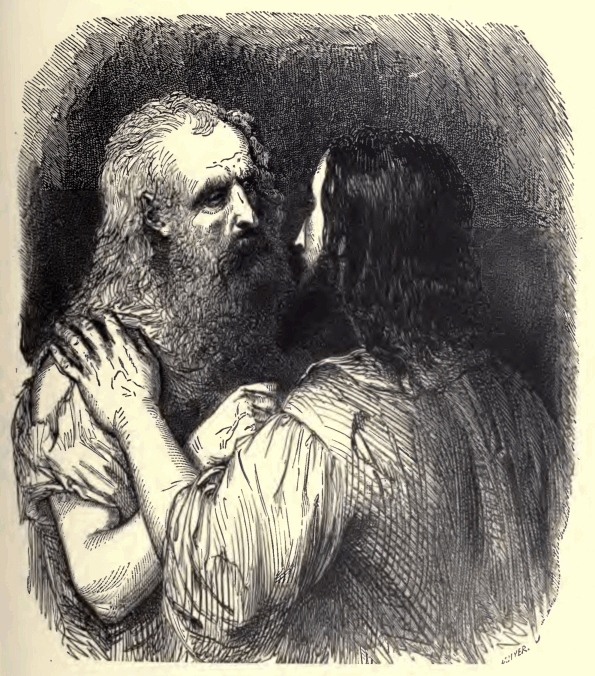
\includegraphics[width=\textwidth]{0201m.jpg}
\end{figure}

“Oh, how I should like to see these products of your industry and
patience.”

“Well, in the first place, here is my chisel.”

So saying, he displayed a sharp strong blade, with a handle made of
beechwood.

“And with what did you contrive to make that?” inquired Dantès.

“With one of the clamps of my bedstead; and this very tool has sufficed
me to hollow out the road by which I came hither, a distance of about
fifty feet.”

“Fifty feet!” responded Dantès, almost terrified.

“Do not speak so loud, young man—don’t speak so loud. It frequently
occurs in a state prison like this, that persons are stationed outside
the doors of the cells purposely to overhear the conversation of the
prisoners.”

“But they believe I am shut up alone here.”

“That makes no difference.”

“And you say that you dug your way a distance of fifty feet to get
here?”

“I do; that is about the distance that separates your chamber from
mine; only, unfortunately, I did not curve aright; for want of the
necessary geometrical instruments to calculate my scale of proportion,
instead of taking an ellipsis of forty feet, I made it fifty. I
expected, as I told you, to reach the outer wall, pierce through it,
and throw myself into the sea; I have, however, kept along the corridor
on which your chamber opens, instead of going beneath it. My labor is
all in vain, for I find that the corridor looks into a courtyard filled
with soldiers.”

“That’s true,” said Dantès; “but the corridor you speak of only bounds
\textit{one} side of my cell; there are three others—do you know anything of
their situation?”

“This one is built against the solid rock, and it would take ten
experienced miners, duly furnished with the requisite tools, as many
years to perforate it. This adjoins the lower part of the governor’s
apartments, and were we to work our way through, we should only get
into some lock-up cellars, where we must necessarily be recaptured. The
fourth and last side of your cell faces on—faces on—stop a minute, now
where does it face?”

The wall of which he spoke was the one in which was fixed the loophole
by which light was admitted to the chamber. This loophole, which
gradually diminished in size as it approached the outside, to an
opening through which a child could not have passed, was, for better
security, furnished with three iron bars, so as to quiet all
apprehensions even in the mind of the most suspicious jailer as to the
possibility of a prisoner’s escape. As the stranger asked the question,
he dragged the table beneath the window.

“Climb up,” said he to Dantès.

The young man obeyed, mounted on the table, and, divining the wishes of
his companion, placed his back securely against the wall and held out
both hands. The stranger, whom as yet Dantès knew only by the number of
his cell, sprang up with an agility by no means to be expected in a
person of his years, and, light and steady on his feet as a cat or a
lizard, climbed from the table to the outstretched hands of Dantès, and
from them to his shoulders; then, bending double, for the ceiling of
the dungeon prevented him from holding himself erect, he managed to
slip his head between the upper bars of the window, so as to be able to
command a perfect view from top to bottom.

An instant afterwards he hastily drew back his head, saying, “I thought
so!” and sliding from the shoulders of Dantès as dextrously as he had
ascended, he nimbly leaped from the table to the ground.

“What was it that you thought?” asked the young man anxiously, in his
turn descending from the table.

The elder prisoner pondered the matter. “Yes,” said he at length, “it
is so. This side of your chamber looks out upon a kind of open gallery,
where patrols are continually passing, and sentries keep watch day and
night.”

“Are you quite sure of that?”

“Certain. I saw the soldier’s shape and the top of his musket; that
made me draw in my head so quickly, for I was fearful he might also see
me.”

“Well?” inquired Dantès.

“You perceive then the utter impossibility of escaping through your
dungeon?”

“Then——” pursued the young man eagerly.

“Then,” answered the elder prisoner, “the will of God be done!” And as
the old man slowly pronounced those words, an air of profound
resignation spread itself over his careworn countenance. Dantès gazed
on the man who could thus philosophically resign hopes so long and
ardently nourished with an astonishment mingled with admiration.

“Tell me, I entreat of you, who and what you are?” said he at length.
“Never have I met with so remarkable a person as yourself.”

“Willingly,” answered the stranger; “if, indeed, you feel any curiosity
respecting one, now, alas, powerless to aid you in any way.”

“Say not so; you can console and support me by the strength of your own
powerful mind. Pray let me know who you really are?”

The stranger smiled a melancholy smile. “Then listen,” said he. “I am
the Abbé Faria, and have been imprisoned as you know in this Château
d’If since the year 1811; previously to which I had been confined for
three years in the fortress of Fenestrelle. In the year 1811 I was
transferred to Piedmont in France. It was at this period I learned that
the destiny which seemed subservient to every wish formed by Napoleon,
had bestowed on him a son, named king of Rome even in his cradle. I was
very far then from expecting the change you have just informed me of;
namely, that four years afterwards, this colossus of power would be
overthrown. Then who reigns in France at this moment—Napoleon II.?”

“No, Louis XVIII.”

“The brother of Louis XVI.! How inscrutable are the ways of
Providence—for what great and mysterious purpose has it pleased Heaven
to abase the man once so elevated, and raise up him who was so abased?”

Dantès’ whole attention was riveted on a man who could thus forget his
own misfortunes while occupying himself with the destinies of others.

“Yes, yes,” continued he, “’Twill be the same as it was in England.
After Charles I., Cromwell; after Cromwell, Charles II., and then James
II., and then some son-in-law or relation, some Prince of Orange, a
stadtholder who becomes a king. Then new concessions to the people,
then a constitution, then liberty. Ah, my friend!” said the abbé,
turning towards Dantès, and surveying him with the kindling gaze of a
prophet, “you are young, you will see all this come to pass.”

“Probably, if ever I get out of prison!”

“True,” replied Faria, “we are prisoners; but I forget this sometimes,
and there are even moments when my mental vision transports me beyond
these walls, and I fancy myself at liberty.”

“But wherefore are you here?”

“Because in 1807 I dreamed of the very plan Napoleon tried to realize
in 1811; because, like Machiavelli, I desired to alter the political
face of Italy, and instead of allowing it to be split up into a
quantity of petty principalities, each held by some weak or tyrannical
ruler, I sought to form one large, compact, and powerful empire; and,
lastly, because I fancied I had found my Cæsar Borgia in a crowned
simpleton, who feigned to enter into my views only to betray me. It was
the plan of Alexander VI. and Clement VII., but it will never succeed
now, for they attempted it fruitlessly, and Napoleon was unable to
complete his work. Italy seems fated to misfortune.” And the old man
bowed his head.

Dantès could not understand a man risking his life for such matters.
Napoleon certainly he knew something of, inasmuch as he had seen and
spoken with him; but of Clement VII. and Alexander VI. he knew nothing.

“Are you not,” he asked, “the priest who here in the Château d’If is
generally thought to be—ill?”

“Mad, you mean, don’t you?”

“I did not like to say so,” answered Dantès, smiling.

“Well, then,” resumed Faria with a bitter smile, “let me answer your
question in full, by acknowledging that I am the poor mad prisoner of
the Château d’If, for many years permitted to amuse the different
visitors with what is said to be my insanity; and, in all probability,
I should be promoted to the honor of making sport for the children, if
such innocent beings could be found in an abode devoted like this to
suffering and despair.”

Dantès remained for a short time mute and motionless; at length he
said:

“Then you abandon all hope of escape?”

“I perceive its utter impossibility; and I consider it impious to
attempt that which the Almighty evidently does not approve.”

“Nay, be not discouraged. Would it not be expecting too much to hope to
succeed at your first attempt? Why not try to find an opening in
another direction from that which has so unfortunately failed?”

“Alas, it shows how little notion you can have of all it has cost me to
effect a purpose so unexpectedly frustrated, that you talk of beginning
over again. In the first place, I was four years making the tools I
possess, and have been two years scraping and digging out earth, hard
as granite itself; then what toil and fatigue has it not been to remove
huge stones I should once have deemed impossible to loosen. Whole days
have I passed in these Titanic efforts, considering my labor well
repaid if, by night-time I had contrived to carry away a square inch of
this hard-bound cement, changed by ages into a substance unyielding as
the stones themselves; then to conceal the mass of earth and rubbish I
dug up, I was compelled to break through a staircase, and throw the
fruits of my labor into the hollow part of it; but the well is now so
completely choked up, that I scarcely think it would be possible to add
another handful of dust without leading to discovery. Consider also
that I fully believed I had accomplished the end and aim of my
undertaking, for which I had so exactly husbanded my strength as to
make it just hold out to the termination of my enterprise; and now, at
the moment when I reckoned upon success, my hopes are forever dashed
from me. No, I repeat again, that nothing shall induce me to renew
attempts evidently at variance with the Almighty’s pleasure.”

Dantès held down his head, that the other might not see how joy at the
thought of having a companion outweighed the sympathy he felt for the
failure of the abbé’s plans.

The abbé sank upon Edmond’s bed, while Edmond himself remained
standing. Escape had never once occurred to him. There are, indeed,
some things which appear so impossible that the mind does not dwell on
them for an instant. To undermine the ground for fifty feet—to devote
three years to a labor which, if successful, would conduct you to a
precipice overhanging the sea—to plunge into the waves from the height
of fifty, sixty, perhaps a hundred feet, at the risk of being dashed to
pieces against the rocks, should you have been fortunate enough to have
escaped the fire of the sentinels; and even, supposing all these perils
past, then to have to swim for your life a distance of at least three
miles ere you could reach the shore—were difficulties so startling and
formidable that Dantès had never even dreamed of such a scheme,
resigning himself rather to death.

But the sight of an old man clinging to life with so desperate a
courage, gave a fresh turn to his ideas, and inspired him with new
courage. Another, older and less strong than he, had attempted what he
had not had sufficient resolution to undertake, and had failed only
because of an error in calculation. This same person, with almost
incredible patience and perseverance, had contrived to provide himself
with tools requisite for so unparalleled an attempt. Another had done
all this; why, then, was it impossible to Dantès? Faria had dug his way
through fifty feet, Dantès would dig a hundred; Faria, at the age of
fifty, had devoted three years to the task; he, who was but half as
old, would sacrifice six; Faria, a priest and savant, had not shrunk
from the idea of risking his life by trying to swim a distance of three
miles to one of the islands—Daume, Rattonneau, or Lemaire; should a
hardy sailor, an experienced diver, like himself, shrink from a similar
task; should he, who had so often for mere amusement’s sake plunged to
the bottom of the sea to fetch up the bright coral branch, hesitate to
entertain the same project? He could do it in an hour, and how many
times had he, for pure pastime, continued in the water for more than
twice as long! At once Dantès resolved to follow the brave example of
his energetic companion, and to remember that what has once been done
may be done again.

After continuing some time in profound meditation, the young man
suddenly exclaimed, “I have found what you were in search of!”

Faria started: “Have you, indeed?” cried he, raising his head with
quick anxiety; “pray, let me know what it is you have discovered?”

“The corridor through which you have bored your way from the cell you
occupy here, extends in the same direction as the outer gallery, does
it not?”

\begin{figure}[ht]
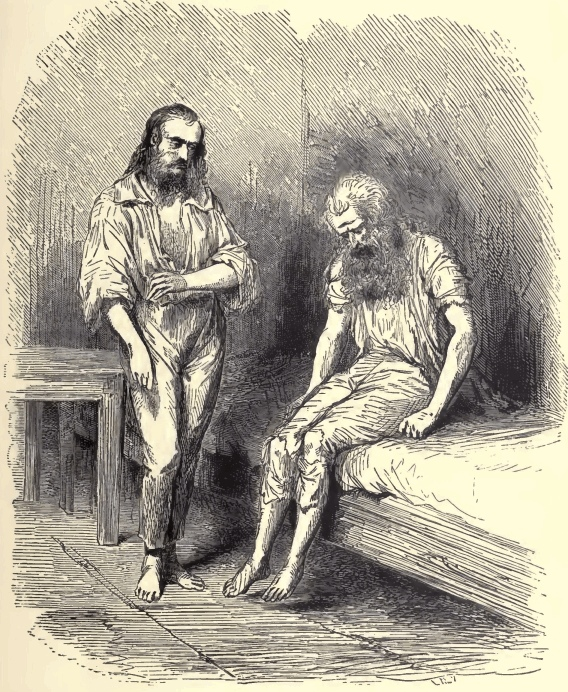
\includegraphics[width=\textwidth]{0207m.jpg}
\end{figure}

“It does.”

“And is not above fifteen feet from it?”

“About that.”

“Well, then, I will tell you what we must do. We must pierce through
the corridor by forming a side opening about the middle, as it were the
top part of a cross. This time you will lay your plans more accurately;
we shall get out into the gallery you have described; kill the sentinel
who guards it, and make our escape. All we require to insure success is
courage, and that you possess, and strength, which I am not deficient
in; as for patience, you have abundantly proved yours—you shall now see
me prove mine.”

“One instant, my dear friend,” replied the abbé; “it is clear you do
not understand the nature of the courage with which I am endowed, and
what use I intend making of my strength. As for patience, I consider
that I have abundantly exercised that in beginning every morning the
task of the night before, and every night renewing the task of the day.
But then, young man (and I pray of you to give me your full attention),
then I thought I could not be doing anything displeasing to the
Almighty in trying to set an innocent being at liberty—one who had
committed no offence, and merited not condemnation.”

“And have your notions changed?” asked Dantès with much surprise; “do
you think yourself more guilty in making the attempt since you have
encountered me?”

“No; neither do I wish to incur guilt. Hitherto I have fancied myself
merely waging war against circumstances, not men. I have thought it no
sin to bore through a wall, or destroy a staircase; but I cannot so
easily persuade myself to pierce a heart or take away a life.”

A slight movement of surprise escaped Dantès.

“Is it possible,” said he, “that where your liberty is at stake you can
allow any such scruple to deter you from obtaining it?”

“Tell me,” replied Faria, “what has hindered you from knocking down
your jailer with a piece of wood torn from your bedstead, dressing
yourself in his clothes, and endeavoring to escape?”

“Simply the fact that the idea never occurred to me,” answered Dantès.

“Because,” said the old man, “the natural repugnance to the commission
of such a crime prevented you from thinking of it; and so it ever is
because in simple and allowable things our natural instincts keep us
from deviating from the strict line of duty. The tiger, whose nature
teaches him to delight in shedding blood, needs but the sense of smell
to show him when his prey is within his reach, and by following this
instinct he is enabled to measure the leap necessary to permit him to
spring on his victim; but man, on the contrary, loathes the idea of
blood—it is not alone that the laws of social life inspire him with a
shrinking dread of taking life; his natural construction and
physiological formation——”

Dantès was confused and silent at this explanation of the thoughts
which had unconsciously been working in his mind, or rather soul; for
there are two distinct sorts of ideas, those that proceed from the head
and those that emanate from the heart.

\begin{figure}[h]
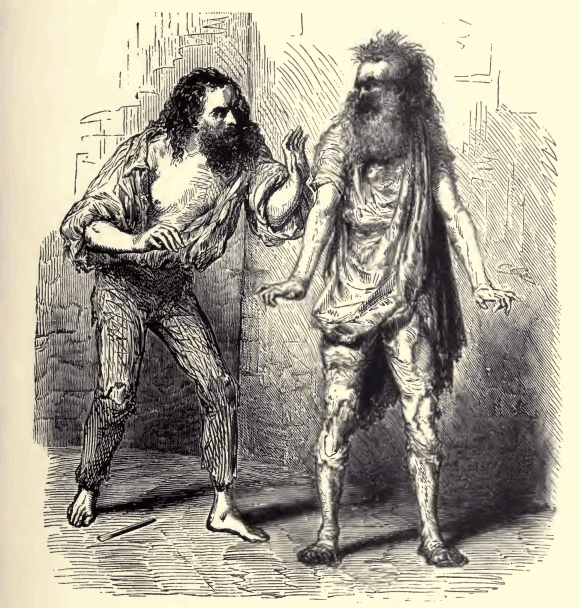
\includegraphics[width=\textwidth]{0209m.jpg}
\end{figure}

“Since my imprisonment,” said Faria, “I have thought over all the most
celebrated cases of escape on record. They have rarely been successful.
Those that have been crowned with full success have been long meditated
upon, and carefully arranged; such, for instance, as the escape of the
Duc de Beaufort from the Château de Vincennes, that of the Abbé
Dubuquoi from For l’Evêque; of Latude from the Bastille. Then there are
those for which chance sometimes affords opportunity, and those are the
best of all. Let us, therefore, wait patiently for some favorable
moment, and when it presents itself, profit by it.”

“Ah,” said Dantès, “you might well endure the tedious delay; you were
constantly employed in the task you set yourself, and when weary with
toil, you had your hopes to refresh and encourage you.”

“I assure you,” replied the old man, “I did not turn to that source for
recreation or support.”

“What did you do then?”

“I wrote or studied.”

“Were you then permitted the use of pens, ink, and paper?”

“Oh, no,” answered the abbé; “I had none but what I made for myself.”

“You made paper, pens and ink?”

“Yes.”

Dantès gazed with admiration, but he had some difficulty in believing.
Faria saw this.

“When you pay me a visit in my cell, my young friend,” said he, “I will
show you an entire work, the fruits of the thoughts and reflections of
my whole life; many of them meditated over in the shades of the
Colosseum at Rome, at the foot of St. Mark’s column at Venice, and on
the borders of the Arno at Florence, little imagining at the time that
they would be arranged in order within the walls of the Château d’If.
The work I speak of is called \textit{A Treatise on the Possibility of a
General Monarchy in Italy}, and will make one large quarto volume.”

“And on what have you written all this?”

“On two of my shirts. I invented a preparation that makes linen as
smooth and as easy to write on as parchment.”

“You are, then, a chemist?”

“Somewhat; I know Lavoisier, and was the intimate friend of Cabanis.”

“But for such a work you must have needed books—had you any?”

“I had nearly five thousand volumes in my library at Rome; but after
reading them over many times, I found out that with one hundred and
fifty well-chosen books a man possesses, if not a complete summary of
all human knowledge, at least all that a man need really know. I
devoted three years of my life to reading and studying these one
hundred and fifty volumes, till I knew them nearly by heart; so that
since I have been in prison, a very slight effort of memory has enabled
me to recall their contents as readily as though the pages were open
before me. I could recite you the whole of Thucydides, Xenophon,
Plutarch, Titus Livius, Tacitus, Strada, Jornandes, Dante, Montaigne,
Shakespeare, Spinoza, Machiavelli, and Bossuet. I name only the most
important.”

“You are, doubtless, acquainted with a variety of languages, so as to
have been able to read all these?”

“Yes, I speak five of the modern tongues—that is to say, German,
French, Italian, English, and Spanish; by the aid of ancient Greek I
learned modern Greek—I don’t speak it so well as I could wish, but I am
still trying to improve myself.”

“Improve yourself!” repeated Dantès; “why, how can you manage to do
so?”

“Why, I made a vocabulary of the words I knew; turned, returned, and
arranged them, so as to enable me to express my thoughts through their
medium. I know nearly one thousand words, which is all that is
absolutely necessary, although I believe there are nearly one hundred
thousand in the dictionaries. I cannot hope to be very fluent, but I
certainly should have no difficulty in explaining my wants and wishes;
and that would be quite as much as I should ever require.”

Stronger grew the wonder of Dantès, who almost fancied he had to do
with one gifted with supernatural powers; still hoping to find some
imperfection which might bring him down to a level with human beings,
he added, “Then if you were not furnished with pens, how did you manage
to write the work you speak of?”

“I made myself some excellent ones, which would be universally
preferred to all others if once known. You are aware what huge whitings
are served to us on \textit{maigre} days. Well, I selected the cartilages of
the heads of these fishes, and you can scarcely imagine the delight
with which I welcomed the arrival of each Wednesday, Friday, and
Saturday, as affording me the means of increasing my stock of pens; for
I will freely confess that my historical labors have been my greatest
solace and relief. While retracing the past, I forget the present; and
traversing at will the path of history I cease to remember that I am
myself a prisoner.”

“But the ink,” said Dantès; “of what did you make your ink?”

“There was formerly a fireplace in my dungeon,” replied Faria, “but it
was closed up long ere I became an occupant of this prison. Still, it
must have been many years in use, for it was thickly covered with a
coating of soot; this soot I dissolved in a portion of the wine brought
to me every Sunday, and I assure you a better ink cannot be desired.
For very important notes, for which closer attention is required, I
pricked one of my fingers, and wrote with my own blood.”

“And when,” asked Dantès, “may I see all this?”

“Whenever you please,” replied the abbé.

“Oh, then let it be directly!” exclaimed the young man.

“Follow me, then,” said the abbé, as he re-entered the subterranean
passage, in which he soon disappeared, followed by Dantès.
